\chapter{RESULTS}\label{resultsChapter}

This chapter would focus on summarize the results of this thesis. Some of those results were already discussed. For example, the implementation of a flocking algorithm in OpenCL was discussed in Section~\ref{flocksection}, and the development of the UI modifier for the Blender Game Engine discussed in Section~\ref{modifiersection}. 

In this chapter demonstrations using the RTPS library and the RTPS modifier are going to be presented.

% demos
\section{Demos}

\subsection{Symmetry of the Basic Rules}
As discussed before the three basic rules of flocking are: \textit{separation}, \textit{alignment}, and \textit{cohesion}. We can see that running demonstrations of each of the rules by themselves, an important property between the rules is preserved. This property is symmetry. When we said that a rule is symmetric, we mean that when starting from a shape like a square where all points are distributed equally from the origin which is the center of the square, the points are going to be moving equally at each quadrant. This would be symmetry, if the most top right particle moves to the right, the bottom right would also move to the right, and the top and bottom left particles would move to the left, respectively.

We are going to start from an squared initial position showed in Figure~\ref{alignRule}. From there, the symmetric moves of \textit{separation} and \textit{cohesion} are shown in Figure~\ref{sepRule} and~\ref{cohRule}, respectively. These figures show 144 boids in a centralized square inside a $5$x$5$x$5$ box.

When running \textit{separation}, its weight was the only one with a value of one, the weights for the other rules were set to zero. We did the same, when we were testing cohesion.

Since, the rendering methods that are available at this moment in RTPS are points, sprites, screen space and spheres we are not able to present a visual demo on the symmetry of alignment. Although \textit{alignment} is also symmetric. Consider starting with the same initial conditions than in Figure~\ref{alignRule}, what only matters for \textit{alignment} is the velocities. If starting with velocities equal to zero, the particles would be aligned and pointing to the direction since the demo starts. Recalling that we only want to prove that the rules are symmetric assuming that they start from a symmetric configuration, and we only assure that the symmetry is preserved.

% alignment
\begin{figure}[htbp]
\begin{center}
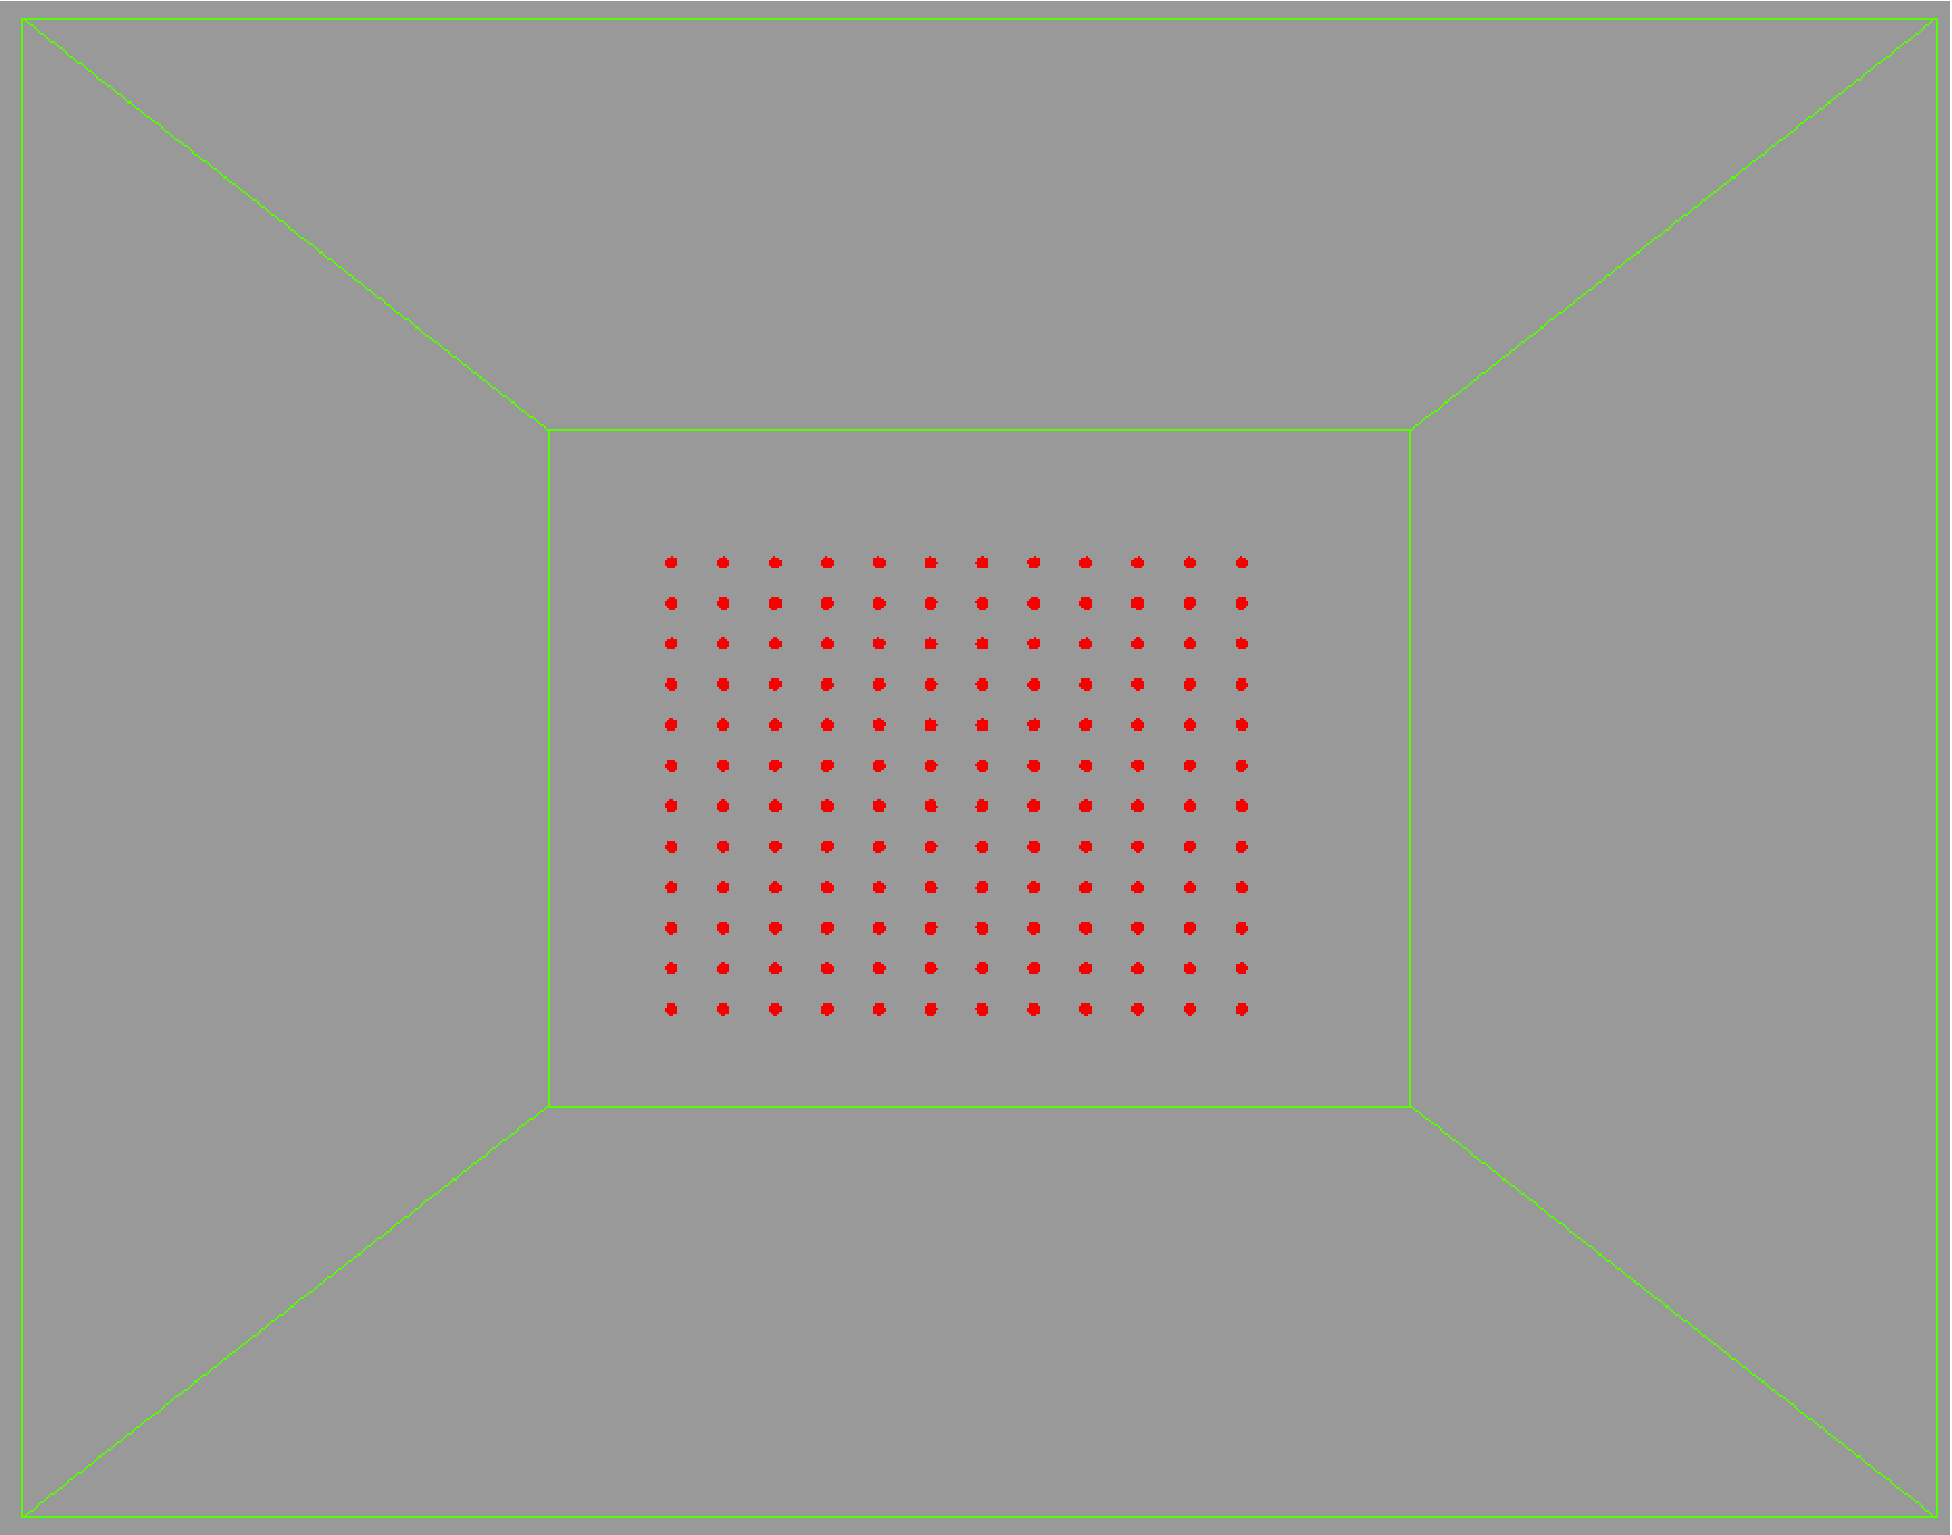
\includegraphics[scale=0.5]{figures/align.pdf}
\caption{Initial state of the boids: the weights for each of the rules are zero, the boids are initialized equally spaced forming a symmetric square}
\label{alignRule}
\end{center}
\end{figure}

% separation
\begin{figure}[htbp]
\begin{center}$
\begin{array}{cc}
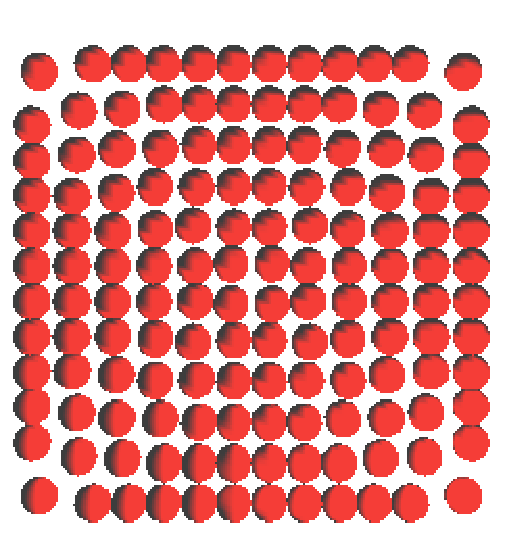
\includegraphics[scale= 0.5]{figures/sep1.pdf} &
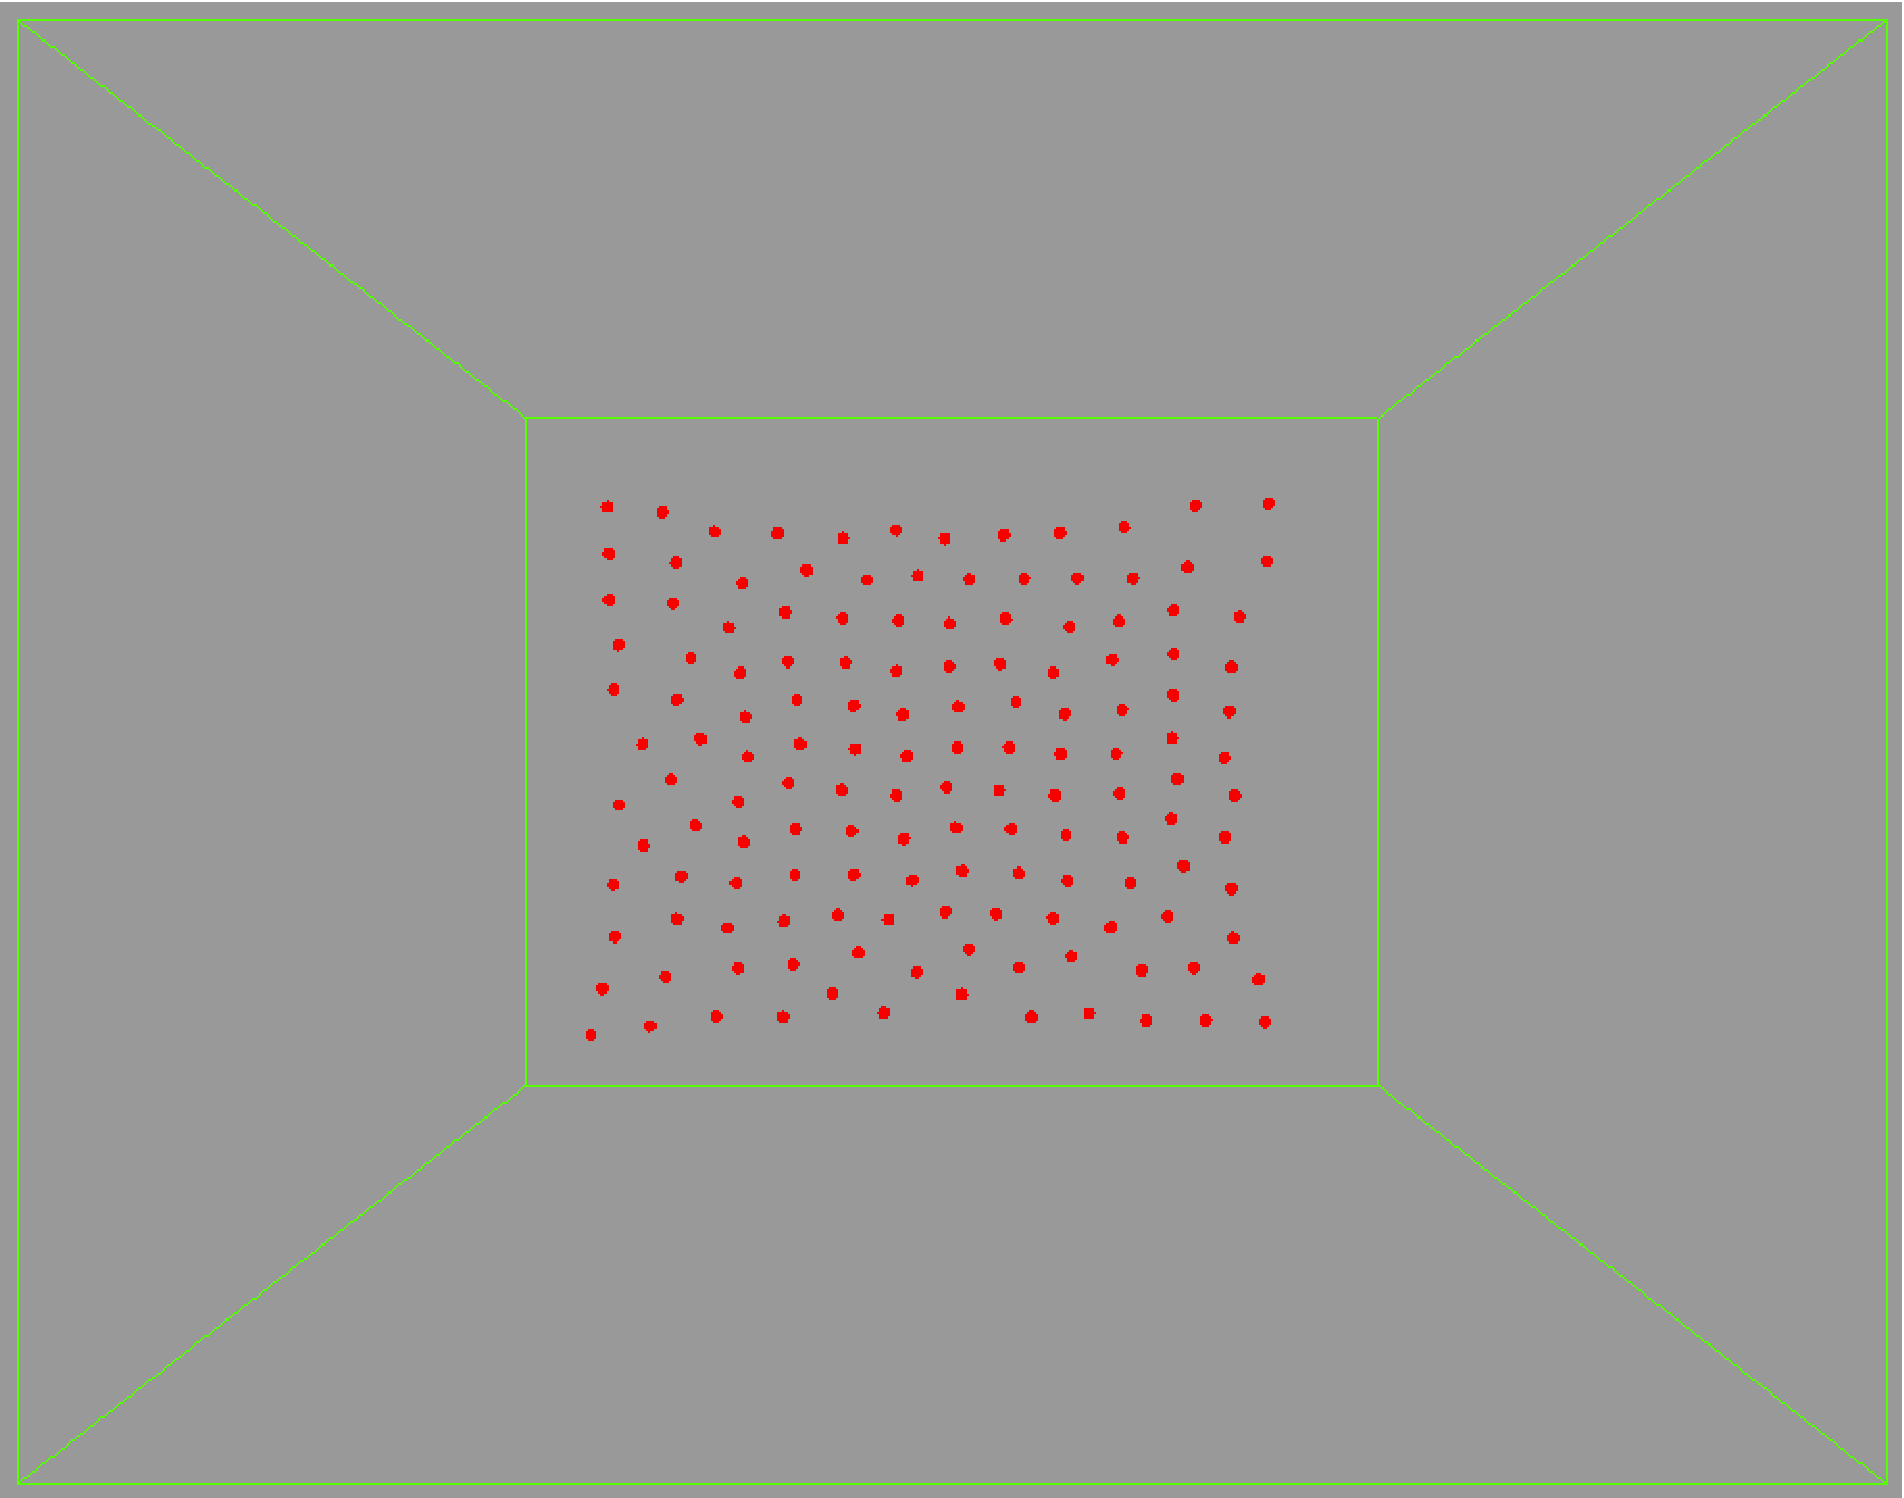
\includegraphics[scale= 0.5]{figures/sep2.pdf}
\end{array}$
\end{center}
\caption{Screenshots of the separation rule: the weight for \textit{separation} was set to 1 while the weights of the other two rules were zero, the boids started to spread out symmetrically}
\label{sepRule}
\end{figure}

% cohesion
\begin{figure}[htbp]
\begin{center}
\begin{tabular}{cc}
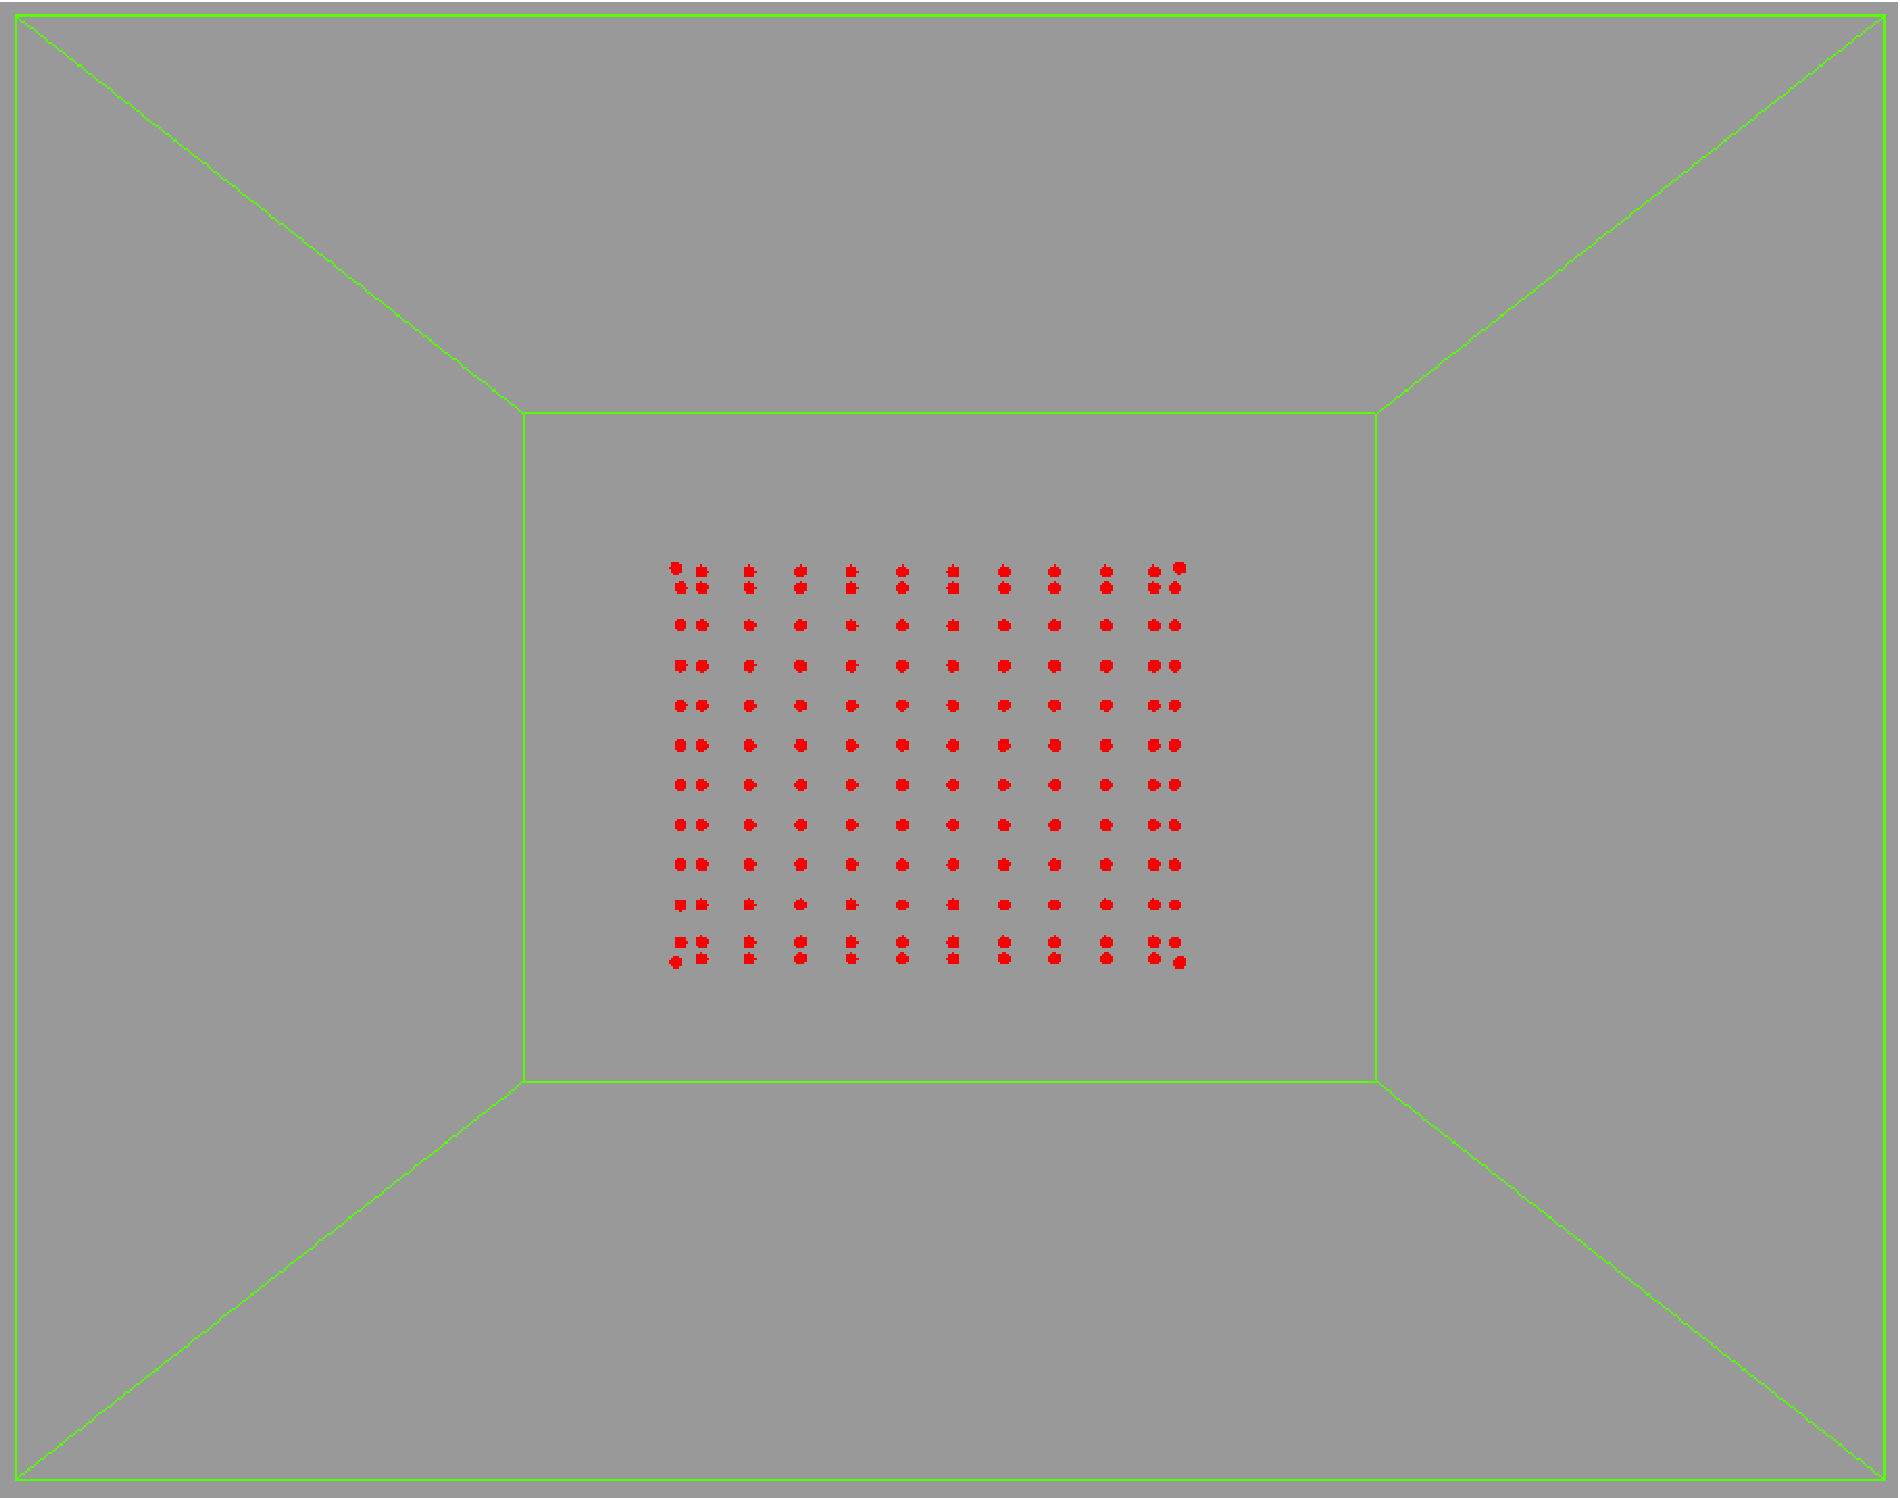
\includegraphics[scale= 0.5]{figures/coh1.pdf} &
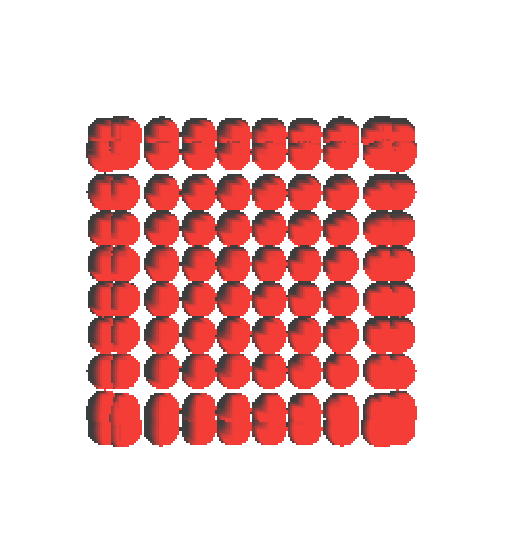
\includegraphics[scale= 0.5]{figures/coh2.pdf} \\

\includegraphics[scale= 0.5]{figures/coh3.pdf} &
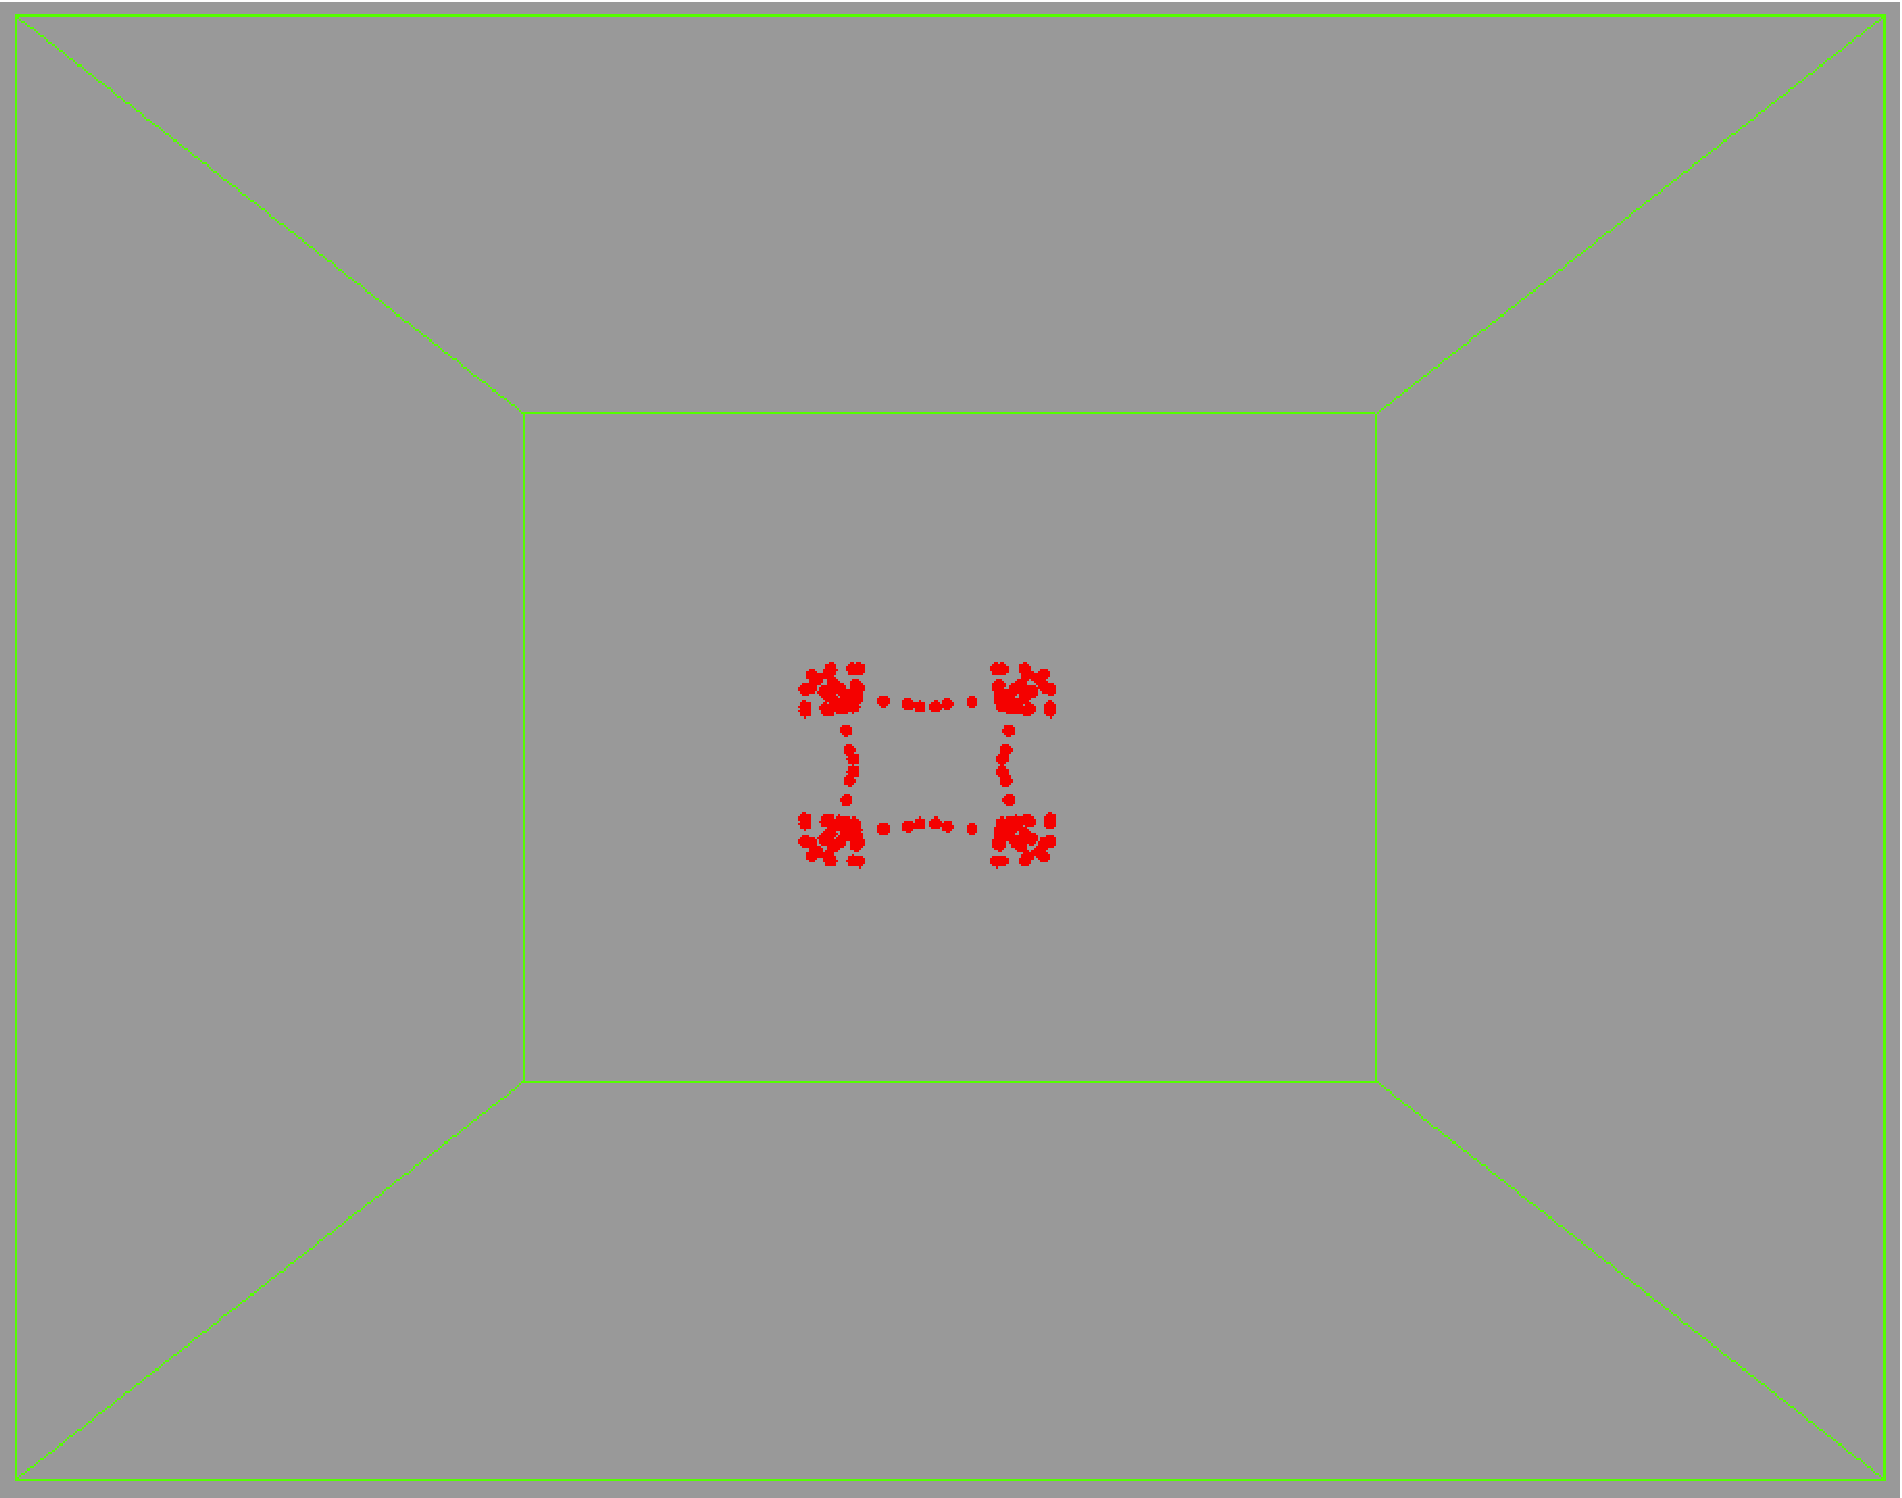
\includegraphics[scale= 0.5]{figures/coh4.pdf}
\end{tabular}
\end{center}
\caption{Screenshots of the cohesion rule: the weight for the \textit{cohesion} rule was set to 1 while the weights for the other two rules were zero, the boids move towards the center causing them to merge symmetrically}
\label{cohRule}
\end{figure}

% Blender demo
\subsection{Blender Demo}
\textcolor{red}{** TODO: missing the Blender demo ***}

\section{Benchmarks}
% mention which kind of hardware I'm using

The flocking OpenCL implementation presented in this thesis was timed. The RTPS library seems to outperform the Blender Boid system. Figure~\ref{plot} show the timings for more than half of a million boids. These boids were represented as spheres in a simple scene with no other objects. Blender was running faster than RTPS when the amount of particles were small, then when big numbers came around, Blender's performance disappears.  We were able to render more than $65K$ boids at $60$ fps and more than half of a million boids at a rate of $10$ fps.

% benchmarks 
\begin{figure}[htbp]
\begin{center}
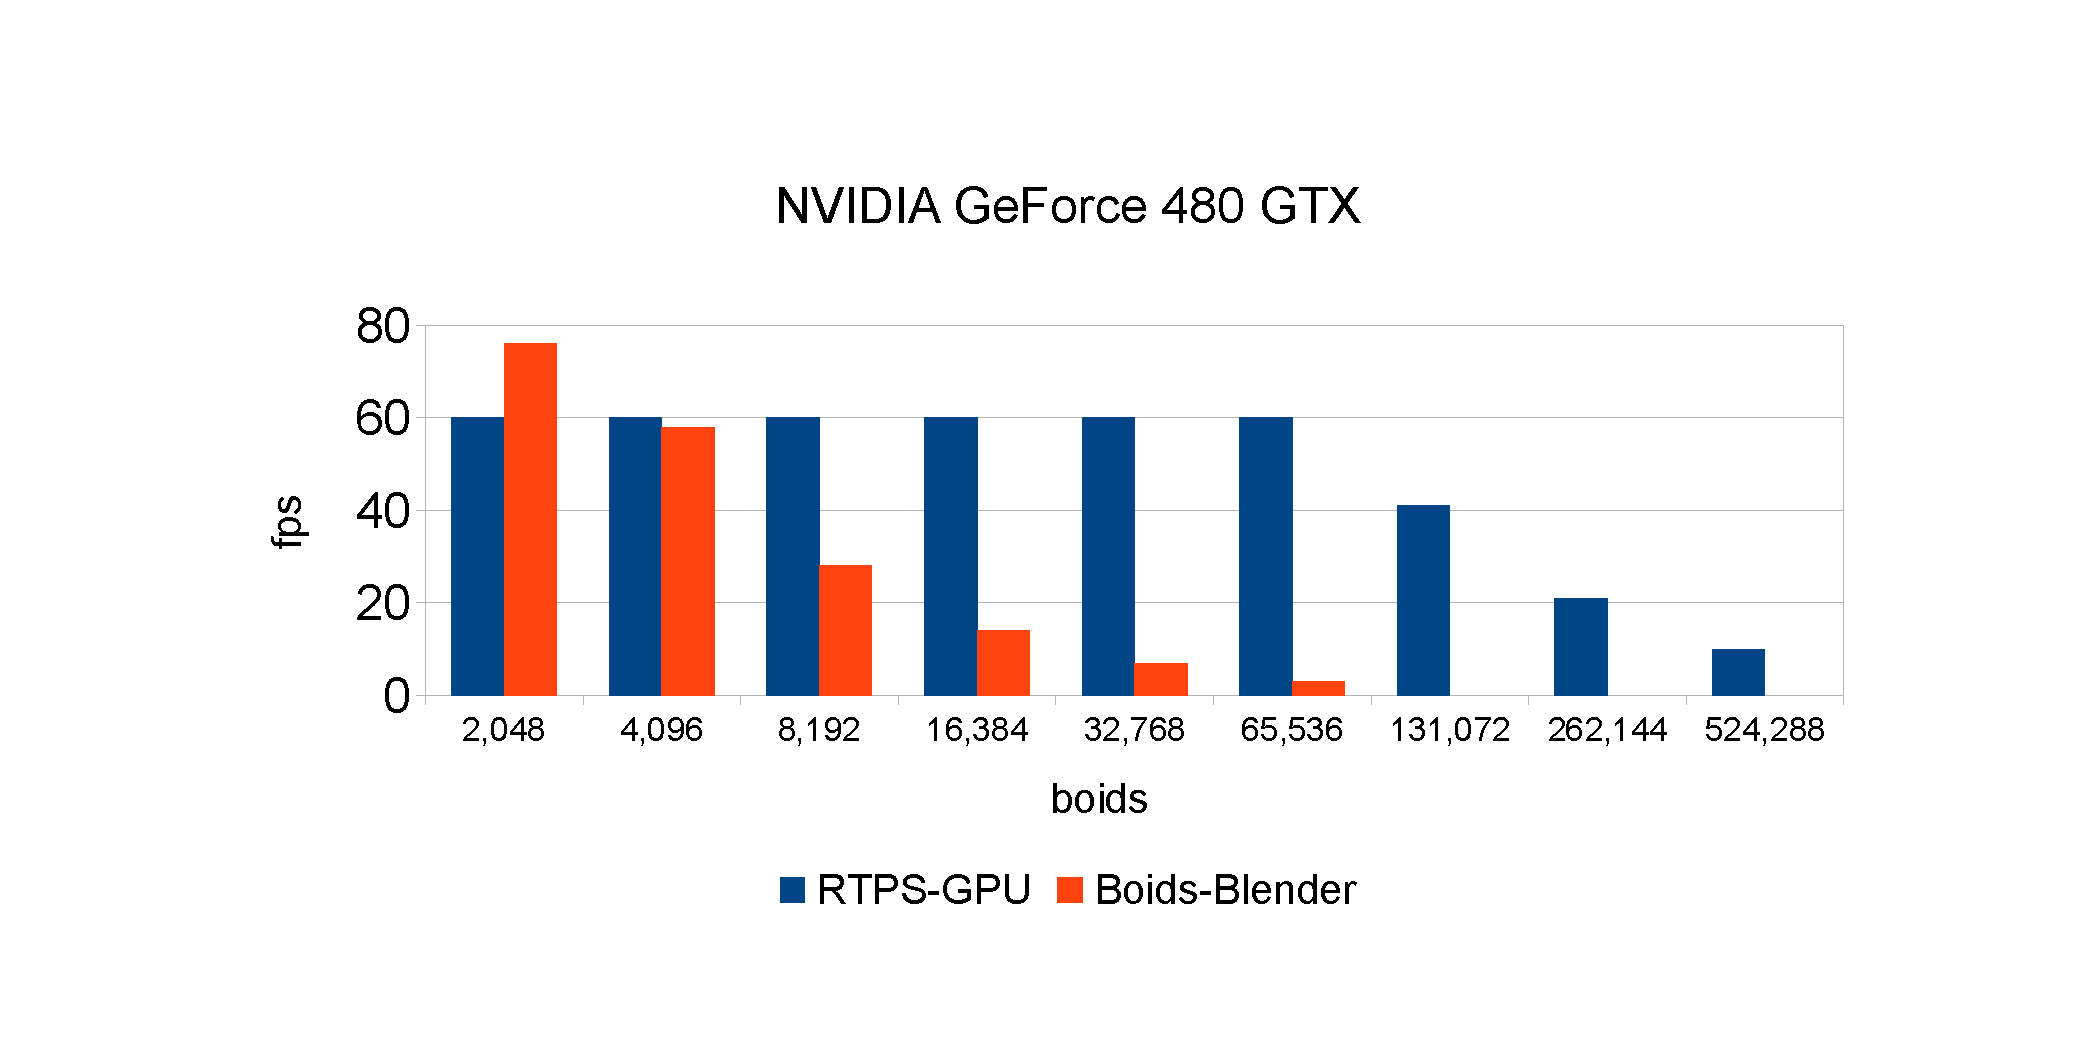
\includegraphics[scale=0.45]{figures/benchmarks.pdf}
\caption{Timings of RTPS modifier and Blender Boids system: the RTPS-GPU implementation outperforms the Blender Boids system}
\label{plot}
\end{center}
\end{figure}

Comparing our performance with some of the benchmarks that were mentioned in Section~\ref{flockingGPU}, our flocking implementation still outperforms them. The library BehaveRT was used to run simulations in real-time and visualization, in that paper Era et al. ran $130K$ boids at 15 fps, we ran more than $131K$ boids at 41 fps. Of course, the timings depend on which hardware they used to get the benchmarks. Our benchmarks were taken in a Dell XXX with a processor XXX, and a NVIDIA GeForce 480 GTX GPU computing device. 

We also measured the inner performance of our flocking implementation in the RTPS library, to do so, we measured the time that took every kernel to be executed. Figure~\ref{kernelBench} shows the timings for the kernels.

\textcolor{red}{TODO: create a chart with the timings per kernel}



